\chapter{Implementation}
\label{chapter6}

\section{Development Environment}
The development of this project was done in various environments, as there was many different aspects to this project.

\subsection{Vive Hardware}
	For this project, the Vive Hardware was set up in a dedicated room (The Virtual Reality Lab in the School of Computing). This allowed development to be done on the HTC Vive without having to set up the sensors and calibrate the hardware everytime that development had to be done, which maximised the amount of development time that was available.\\

\begin{figure}[H]
	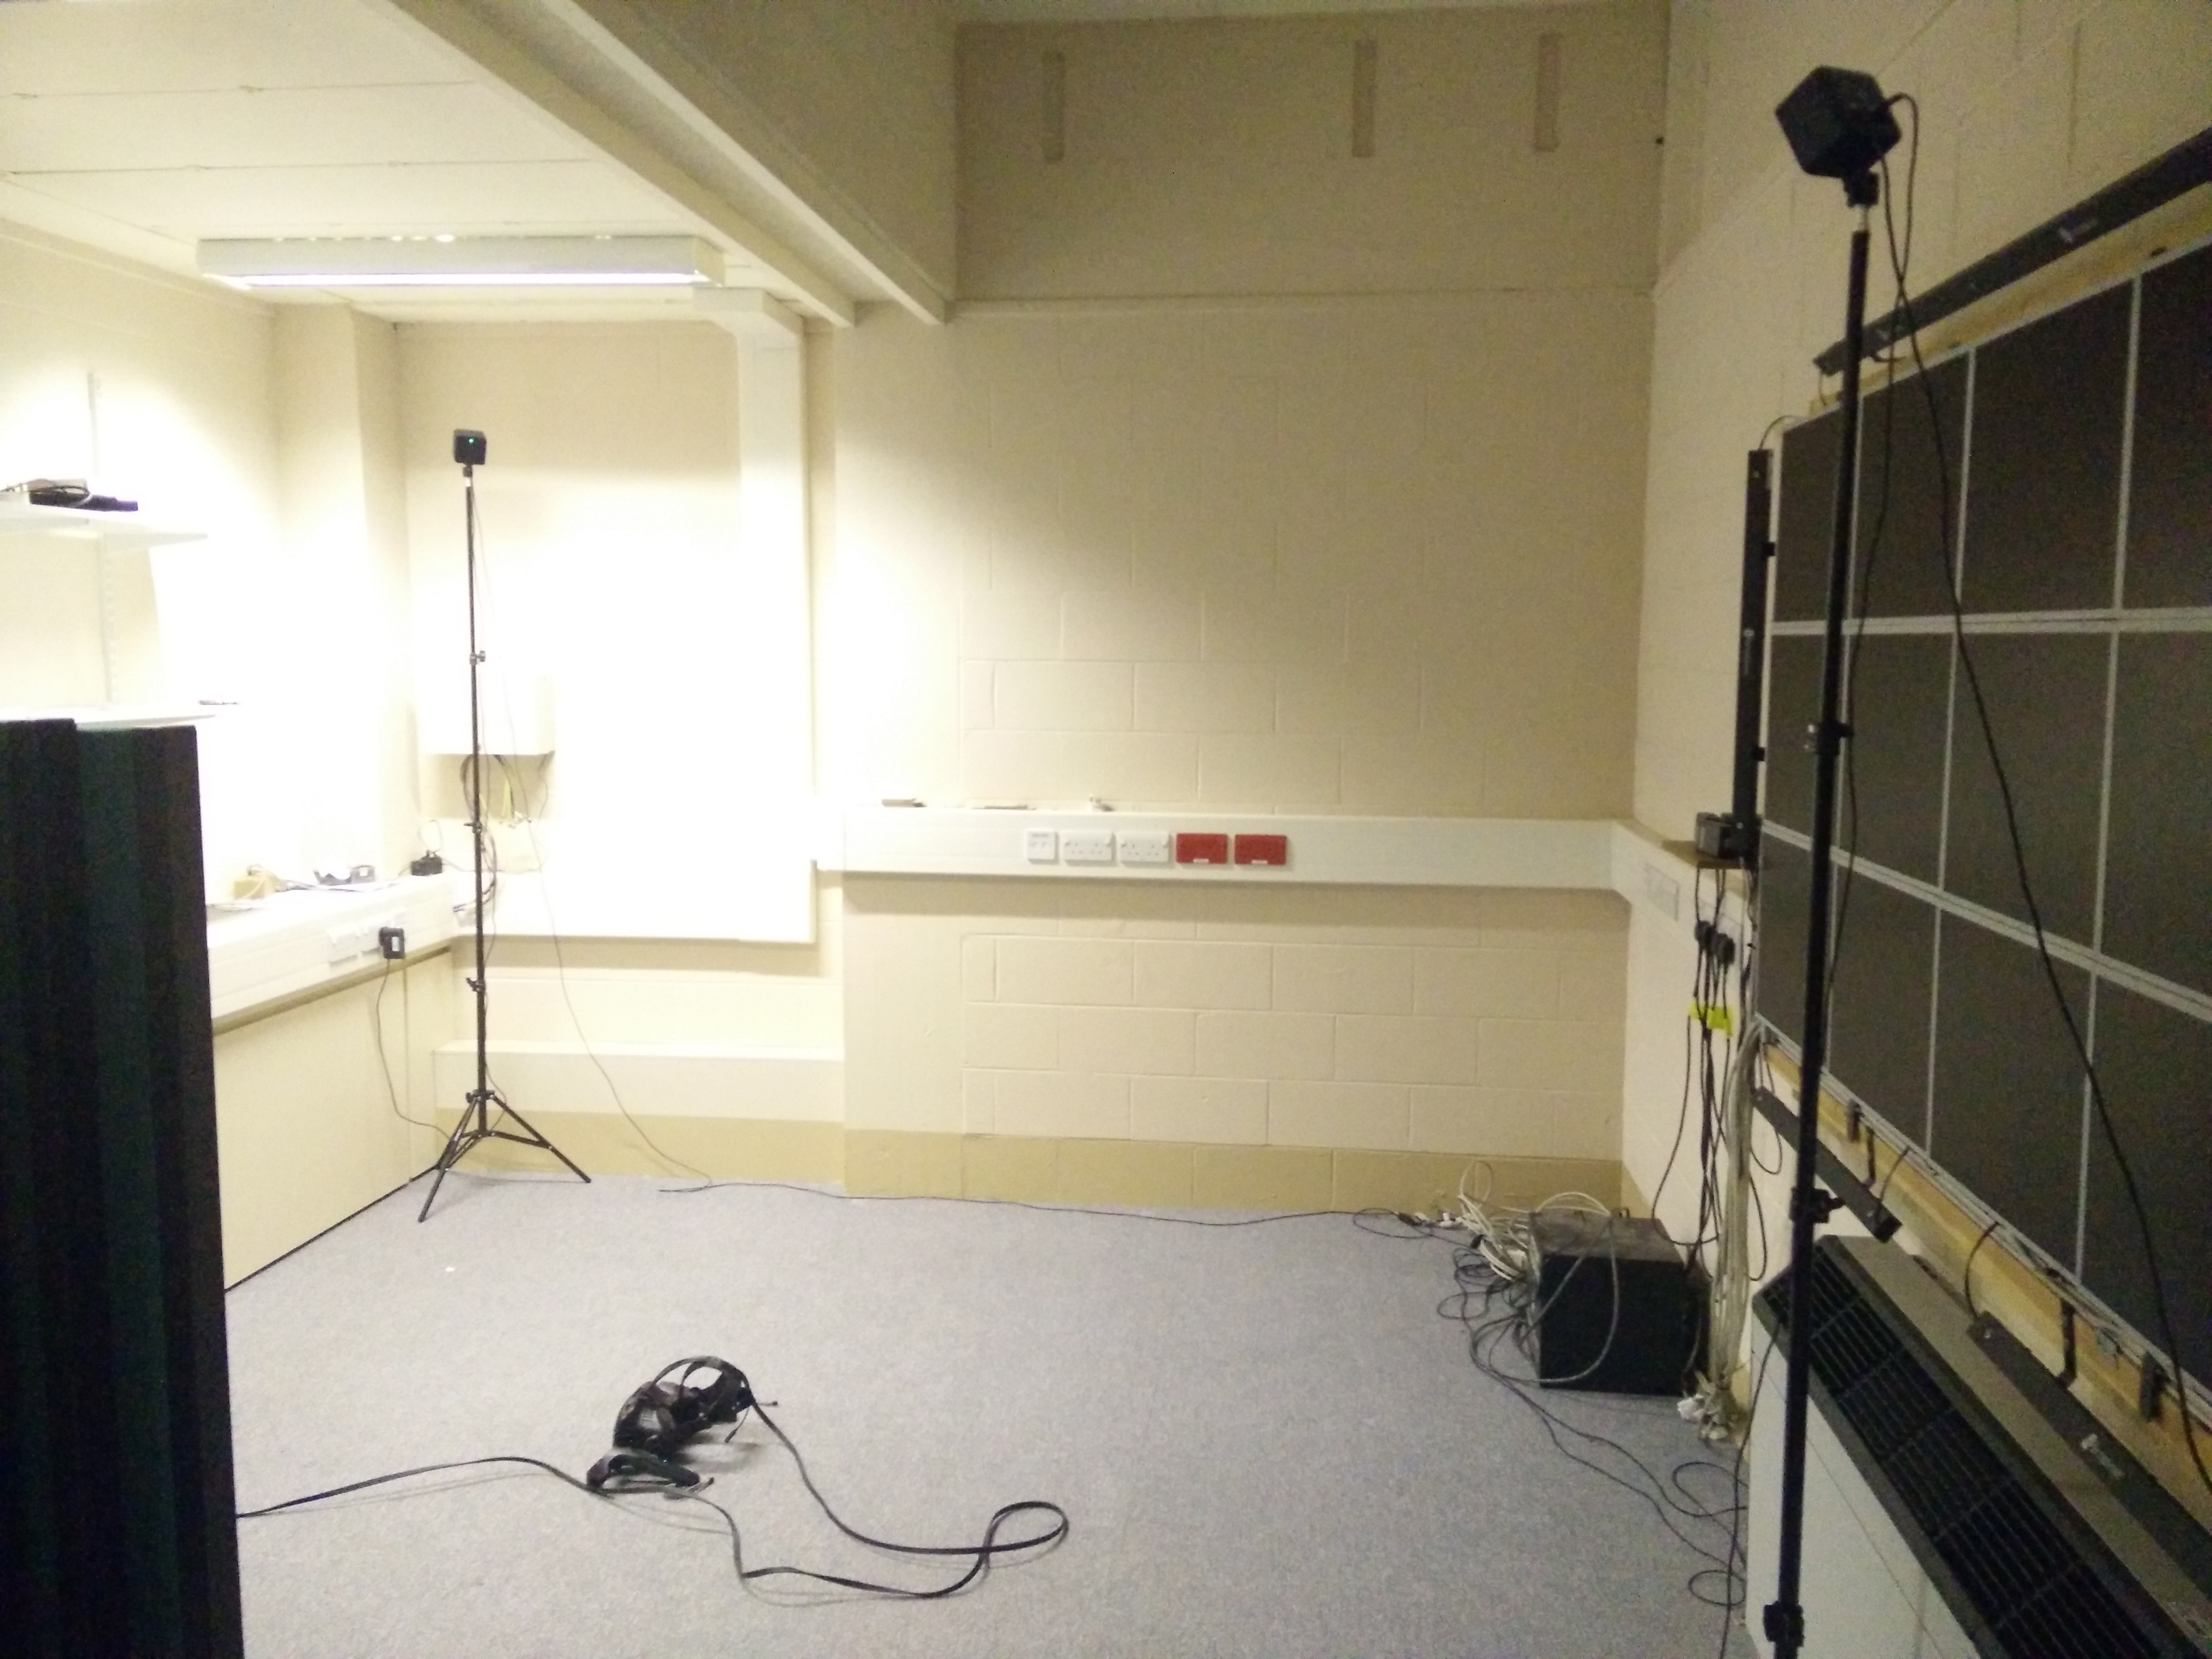
\includegraphics[width=\textwidth]{VRRoom}
	\centering
	\caption{Room used for testing the application}
	\label{fig:VRRoom}
\end{figure}

	This room was chosen as it was unused and met the space requirements for the HTC Vive.

\subsection{Game Engine}
\lipsum[1-1] \cite{parikh1980adaptive}

\subsection{Visual Studio}

\subsection{Windows}

\subsection{Out of Engine Development}
\lipsum[1-1] \cite{parikh1980adaptive}

\section{Random Generation of Graphs, Rivers and Terrain}

%Divide into sub sections as big topic
\subsection{Graph Generation Original Method}
\subsubsection{Point Insertion}
	The original idea to do graph generation was to start with a square, using each corner as a node. These nodes would then be connected as shown in \ref{fig:triangulation1}.\\

\begin{figure}[H]
	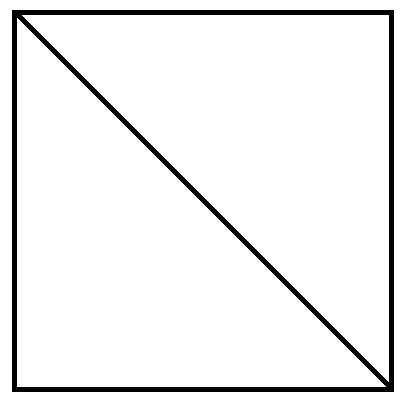
\includegraphics[width=10cm]{triangulation1}
	\centering
	\caption{Original Connections}
	\label{fig:triangulation1}
\end{figure}

	Points would then be inserted into this square, using a random x and y value.  The triangle that this node is in would then be found using the cross product. This was done by checking the cross product of the point and the triangle, for each triangle that is in the graph. The point would then be connected to the corners of this triangle.\\

\begin{figure}[H]
	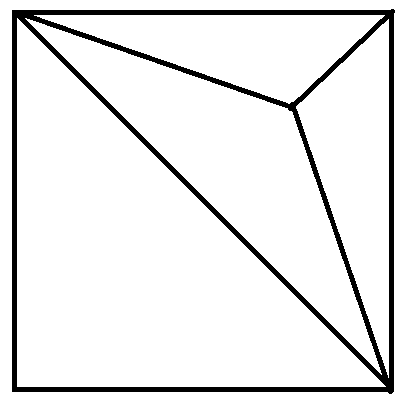
\includegraphics[width=10cm]{triangulation2}
	\centering
	\caption{Example of running the point insertion algorithm for one iteration.}
	\label{fig:triangulation2}
\end{figure}

\begin{figure}[H]
	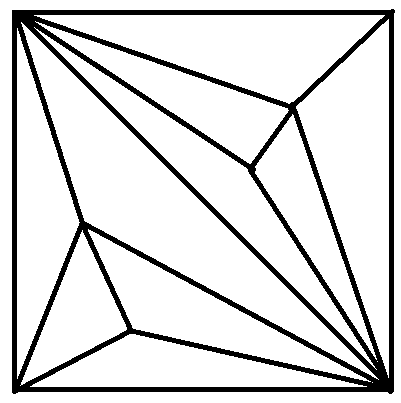
\includegraphics[width=10cm]{triangulation3}
	\centering
	\caption{Example of running the point insertion algorithm for four iterations}
	\label{fig:triangulation3}
\end{figure}

	This approach guaranteed a connected graph to begin with. This approach did not work however as if a node on the bottom-left side of the graph needed to be connected to a node on the top-right side of the graph, the the connection would have to be made through either the top-left node or the bottom-right node, as there was no other way to pass through to the other side of the graph. The approach was then modified slightly to start with an extra node node in the middle of the square, allowing another way to pass through the other side of the graph, this is seen in \ref{fig:triangulation4}.

\begin{figure}[H]
	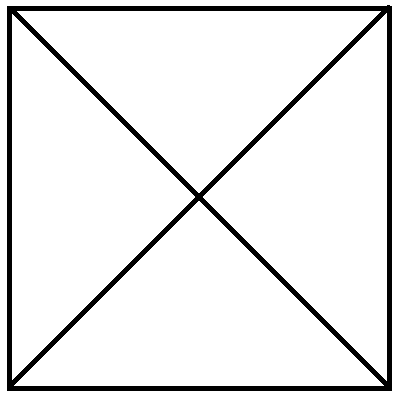
\includegraphics[width=10cm]{triangulation4}
	\centering
	\caption{Image showing the second method's starting connections}
	\label{fig:triangulation4}
\end{figure}
	
	This approach also did not work, as the addition of the extra node did not provide enough of relief for the connections between the two sides of the graph, and the connections would occasionally still go through the top-left or bottom-right node.
The next approach was adding seveeral nodes along the diagonal and connecting them to the corners, similarly to how the middle node was added. The third approach can be seen in \ref{fig:triangulation5}.

\begin{figure}[H]
	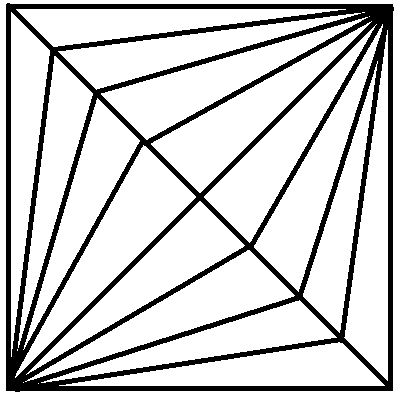
\includegraphics[width=10cm]{triangulation5}
	\centering
	\caption{Image showing the third method's starting connections}
	\label{fig:triangulation5}
\end{figure}

\subsubsection{Connections and Weight Matrix}
	The connections were found by looping through the array that stored the triangles and finding the edges of the triangles. These edges were stored in a connection matrix, to be used when making the weight matrix.\\
	The weight matrix was made using manhattan distance between the two connected points as the heuristic. The manhattan distance is the x distance between the two points plus the distance in the y direction. The manhattan distance was calculated using the following formula:\\

$$Manhattan = (point1.x - point2.x) + (point1.y - point2.y)$$
	
	The manhattan distance then has to be checked to see whether it is positive or not. If it is positive the result is put in element of the matrix representing the first point to the second point, if the result is negative the result is instead placed in the element representing the second point to the first point. This is repeated for each connection in the connection matrix produced before.

\subsubsection{Generating Rivers}
	The river generation starts off with picking the start and end nodes for the rivers, this is done by randomly selecting a set amount of nodes, determined by a variable set in code. 

\subsection{Terrain Generation}

\section{User Interactive Reverse Towers Of Hanoi}
\lipsum[1-1] \cite{parikh1980adaptive}

\section{Graph Flow}

\section{Flow Dependant Flora}
\lipsum[1-1] \cite{parikh1980adaptive}